\subsection{CUDA}

\subsubsection{Basics of CUDA}

\begin{flushleft}
    \textcolor{Green3}{\faIcon{question-circle} \textbf{What is CUDA?}}
\end{flushleft}
\definition{Compute Unified Device Architecture (CUDA)}, is a \textbf{parallel computing platform and Application Programming Interface} (API) \textbf{model} created by NVIDIA. It allows developers to utilize NVIDIA GPUs for general-purpose processing, enabling them to perform a wide range of computations more efficiently than with traditional CPU processing alone.

\highspace
CUDA was introduced with the NVIDIA Tesla architecture, which marked a significant shift in GPU capabilities, enabling general purpose computing on GPUs. \textbf{CUDA is designed to be similar to the \texttt{C} programming language}, making it familiar to many developers. It allows programmers to write code that runs on GPUs using the compute-mode hardware interface.

\highspace
\textbf{CUDA's abstractions are relatively low-level and closely match the performance characteristics and capabilities of modern GPUs}. This design goal helps maintain a low abstraction layer, ensuring that developers can take full advantage of the hardware's potential.

\highspace
Note that \definition{Open Computing Language (OpenCL)} is an open standards version of CUDA that runs on both CPUs and GPUs from multiple vendors. \textbf{While CUDA runs only on NVIDIA GPUs, OpenCL is designed to be more versatile and work on hardware from multiple vendors}.

\highspace
\begin{flushleft}
    \textcolor{Green3}{\faIcon{question-circle} \textbf{CUDA Thread Hierarchy}}
\end{flushleft}
CUDA organizes threads into a hierarchical structure to efficiently manage parallel computations on GPUs. To understand how it works, let's look at it from the deepest level up:
\begin{enumerate}
    \item \textbf{Threads}. Threads (or \definition{CUDA Threads}) are the \textbf{smallest unit of execution} in CUDA. Each thread runs a single instance of a kernel function\footnote{A kernel function in CUDA is a function that runs on the GPU (device) but is called from the CPU (host). These functions are executed by many parallel threads on the GPU}.
    
    Threads are \textbf{identified by their unique thread IDs}, which are used to calculate memory addresses and control decisions.
    

    \item \textbf{Thread Blocks}. Threads are grouped into blocks (called also \definition{CUDA Blocks}). Each block can contain multiple threads that execute concurrently.
    
    \textbf{Threads within the same block can communicate and share data} through shared memory and synchronization primitives like barriers and atomic operations.
    
    The \emph{maximum number} of threads per block is limited by the GPU architecture, typically up to 1024 threads per block.
    
    \label{definition: CUDA Grids}
    \item \textbf{Grids}. Blocks are organized into a grid (called also \definition{CUDA Grids}). A grid is a \textbf{collection of blocks that execute the same kernel function}.
    
    All \textbf{threads in a grid share the same global memory space}.
    
    The grid can be multi-dimensional, allowing for flexible organization of blocks to match the problem's dimensions.
\end{enumerate}
Note that CUDA uses the \texttt{x}, \texttt{y}, and \texttt{z} dimensions for threads, blocks, and grids because this \textbf{multi-dimensional structure} aligns well with many common computational problems. Many computational problems naturally fit into a multi-dimensional space. For example, image processing involves 2D data, and volumetric simulations involve 3D data.

\begin{figure}[!htp]
    \centering
    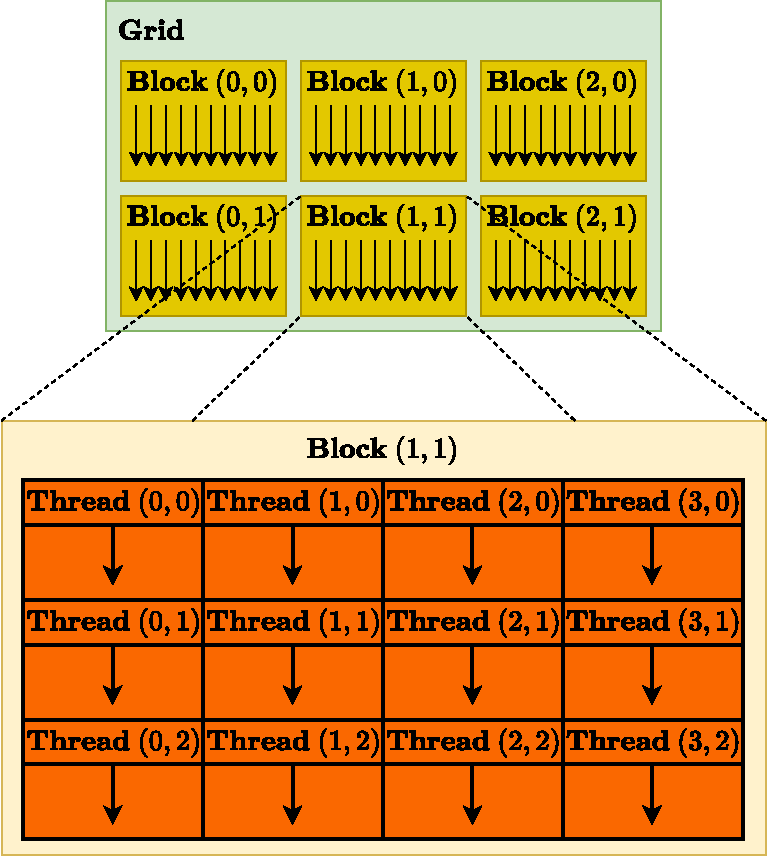
\includegraphics[width=.8\textwidth]{img/CUDA-blocks-grid-threads-1.pdf}
    \caption{The figure shows an example of a CUDA grid consisting of 6 blocks, each block consisting of 12 threads. The number of threads and the number of blocks per column/row are customizable, this is just an example. In total, there are 72 CUDA threads (12 threads per block times 6 blocks in the grid).}
    \label{fig: CUDA example of Grid, Blocks and Threads}
\end{figure}

\begin{flushleft}
    \textcolor{Green3}{\faIcon{calculator} \textbf{CUDA Kernels}}
\end{flushleft}
A \definition{CUDA kernel} is a \textbf{function that gets executed on the GPU}. It contains the parallel portion of the application, which is executed by multiple threads in parallel. Unlike regular C/C++ functions that run on a single thread, CUDA kernels can run thousands of threads simultaneously.

\newpage

\begin{flushleft}
    \textcolor{Green3}{\faIcon{balance-scale} \textbf{Device vs Host}}
\end{flushleft}
In CUDA, there is a term to identify the code that runs on the CPU and GPU.
\begin{definitionbox}[: CUDA Host (CPU)]
    The \definition{CUDA Host} \textbf{refers to the CPU} and its associated memory.

    It is \textbf{responsible for managing the overall program execution}. This includes allocating memory, launching CUDA kernels, and transferring data between the CPU and the GPU.

    It is typically written in the standard programming language used (e.g., C, C++, Java, Python, etc.) and contains the logic for setting up and controlling the execution of CUDA kernels on the device.
\end{definitionbox}

\begin{definitionbox}[: CUDA Device (GPU)]
    The \definition{CUDA Device} \textbf{refers to the GPU} and its associated memory.

    It is \textbf{responsible for running parallel code} (CUDA kernels) and \textbf{performs the bulk of the computation}. This takes advantage of the parallel processing power of the GPU.
    
    The device code (kernels) is written in the CUDA programming language and is designed to run on the multiple parallel cores of the GPU.
\end{definitionbox}

\begin{flushleft}
    \textcolor{Green3}{\faIcon{code} \textbf{Basic CUDA syntax}}
\end{flushleft}
Here is a sample code written in CUDA:
\begin{lstlisting}[language=C++]
#include <cuda_runtime.h>
#include <iostream>
#define Nx 12   $\label{code: CUDA basic - const def 1}$
#define Ny 6    $\label{code: CUDA basic - const def 2}$

// Kernel definition
__global__ void MatAdd( $\label{code: CUDA basic - MatAdd}$
    float A[Ny][Nx], 
    float B[Ny][Nx], 
    float C[Ny][Nx]
) {
    int i = blockIdx.x * blockDim.x + threadIdx.x;$\label{code: CUDA basic - index i}$
    int j = blockIdx.y * blockDim.y + threadIdx.y;$\label{code: CUDA basic - index j}$
    // guard against out of bounds array access
    if (i < N && j < N)                 $\label{code: CUDA basic - if condition}$
        C[i][j] = A[i][j] + B[i][j];    $\label{code: CUDA basic - sum}$
}

int main() {
    // Define the hierarchy
    dim3 threadsPerBlock(4, 3); $\label{code: CUDA basic - threadsPerBlock}$
    dim3 numBlocks(             $\label{code: CUDA basic - numBlocks}$
        Nx / threadsPerBlock.x, 
        Ny / threadsPerBlock.y
    );
    // Kernel invocation
    // Assume matrices A, B, C are already allocated (dim Nx x Ny)
    MatAdd<<<numBlocks, threadsPerBlock>>>(A, B, C); $\label{code: CUDA basic - MatAdd invocation}$
}
\end{lstlisting}
\begin{itemize}
    \item[Rows \ref{code: CUDA basic - const def 1}-\ref{code: CUDA basic - const def 2}] Variables \texttt{Nx} and \texttt{Ny} define the dimensions of the matrices. In this case, they are $12 \times 6$.
    
    \item[Row \ref{code: CUDA basic - threadsPerBlock}] The \texttt{threadsPerBlock} function specifies that each block will have 4\break threads in the \emph{x} dimension and 3 threads in the \emph{y} dimension. In other words, it defines how a block should be composed (see the figure \ref{fig: CUDA example of Grid, Blocks and Threads}).

    \item[Row \ref{code: CUDA basic - numBlocks}] The \texttt{numBlocks} function defines the number of blocks required to cover the entire matrix. The number of blocks is calculated by dividing the matrix dimensions by the number of threads per block in each dimension. In other words, it defines how a grid should be composed (see the figure \ref{fig: CUDA example of Grid, Blocks and Threads}).

    \item[Row \ref{code: CUDA basic - MatAdd invocation}] The execution configuration syntax \texttt{<}\texttt{<}\texttt{<}\texttt{...}\texttt{>}\texttt{>}\texttt{>} is required to specify the number of threads per block and the number of blocks per grid (both numbers can be of type \texttt{int} or \texttt{dim3}).
    
    The function invocation starts the \texttt{MatAdd} kernel with the given grid and block dimensions. This kernel runs on the GPU and performs the matrix addition.

    \item[Row \ref{code: CUDA basic - MatAdd}] Defines a kernel function called \texttt{MatAdd} to be executed on the GPU. The \texttt{\_\_global\_\_} keyword indicates that this is a kernel function.
    
    \item[Rows \ref{code: CUDA basic - index i}-\ref{code: CUDA basic - index j}] Computes the global column index i for each thread. This combines the block index and the thread index within the block to get the overall position.
    
    It also does the same with the j index.

    \item[Row \ref{code: CUDA basic - if condition}] The \texttt{if} condition ensures that the thread does not access out-of-bounds elements in the matrices.
    
    \item[Row \ref{code: CUDA basic - sum}] Finally, it performs the element-wise addition of matrices \texttt{A} and \texttt{B} and stores the result in matrix \texttt{C}.
\end{itemize}
As we said in Figure \ref{fig: CUDA example of Grid, Blocks and Threads} (page \pageref{fig: CUDA example of Grid, Blocks and Threads}), the example spawns 72 CUDA threads.